\documentclass{article}
\usepackage{amsmath,amssymb,graphicx,subfig}

\title{SPL-10473-2011, Inference in Hidden Markov Models with Explicit State Duration Distributions - Response to Reviewers}

\author{Mike Dewar, Chris Wiggins, and Frank Wood}

\begin{document}
\maketitle
We would like to thank the reviewers for their encouraging comments. Below we respond to each reviewer in turn.

\section*{Reviwer 1}

We would like to thank reviewer 1 for the detailed response. We have corrected all the typos mentioned and included the reference on speech synthesis. 

Reviewer 1 has suggested the comparison of our proposed method with Gibbs sampling and the Forward Backward algorithm. We found that we do not have sufficient space to introduce a meaningful comparison to either.  We do here, however, show additional experiments which may help address the reviewer's concern.  We hope that the corrections we made to our prose will be sufficient to explain away many of the reviewer's concerns about the letter.

The first suggested comparison is to a Gibbs sampler.  The Gibbs sampler was too casually mentioned in the original text as Gibbs sampling would require block-sampling in a model augmented with state-change-boundary auxiliary indicator variables.   We have edited the introduction to section 3 and included an additional reference to a paper that samples in this representation and reports the kind of mixing/computational problems that we previously hinted at.

The second suggestion was to use the forward-backward algorithm to perform inference. This requires $O(T^3K^2)$ total cost which is impractical for even the short toy data examples provided in the paper. To escape this cost re-introduces the problem we set out to solve: how to choose a range of possible durations over which to sample. One way to do this, in a manner that is guaranteed not to break, is to allow any duration up to the length of the sequence. Since this is computationally infeasable (see the caption to Figure 4), we can, instead, show the achieved expected joint-likelihood of the model and the data as we increase $d_\mathrm{max}$.  

This unsurprisingly performs poorly exactly as we would expect it to: until $d_\mathrm{max}$ is increased to a value that captures the maximum duration the model fails to adequately capture the true dynamics. Figure \ref{fig} shows the likelihood of 5 samples from the forward backward algorithm as the maximum duration increases, and shows one way that the truncated forward/backward algorithm suffers when the true durations are not in the support of the truncation windows. For comparison, the likelihood of five state sequences sampled using the full beam sampler is shown in red, and the likelihood of the truth is shown in green. While we would enjoy to place this figure in the manuscript, we unfortunately do not have space. Instead, we have placed the code for this experiment in the code repository referenced in the paper. 

\begin{figure}
	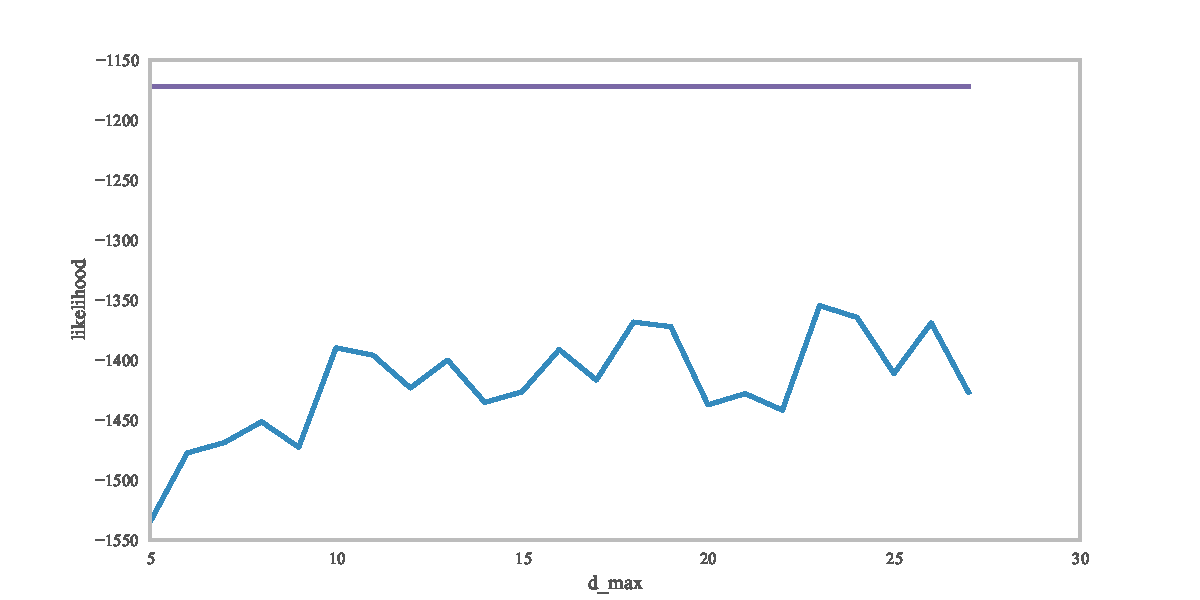
\includegraphics[width=\textwidth]{../pic/likelihood_over_dmax.pdf}
	\caption{Likelihood of sampled state sequences from the forward backward algorithm as the range of possible durations increases (blue lines). Shown for comparison is the likelihood of the true state sequence (green line), and the likelihood of samples from the beam sampler (red lines).}
	\label{fig}
\end{figure}
 
\section*{Reviewer 2}

We thank the reviewer for their comments; we have addressed the typos. The parameter estimation suffers in the second example as we're not able to completely separate the states that have identical observation distributions. The observation distributions all have identical variances, so the separation between states is not due to the observation variance. We do not have an explicit mechanism for controlling state switching in the current algorithm implementation; this would be interesting future work.

Having said this, we are able to show that the algorithm can identify separate states in the second experiment and perform reasonable inference. Examining this specific problem of states that are only seperable by duration would also be interesting future work. It's especially interesting, for example, when studying behaviour in animals (an early motivation for the current paper), as many behaviours are distinguishable by eye only because they spend a different amount of time performing each behaviour: consider `pausing', vs `stunned' vs `dead' - in a video of fruit flies all these behaviours look the same (i.e. have the same observation distribution) over a few frames yet have large duration distribution differences. 

\section*{Reviewer 3}

Reviewer 3 has highlighted two omissions in the paper. The first was that we did not make clear the fact that the Explicit Duration HMM is a type of Hidden Semi Markov Model (HSMM), which is now made clear in the second paragraph of the introduction, along with an additional citation to a review of HSMMs detailing the relationship. The second was that we did not report on the results of the transition rate parameter estimates. While we do not report any detailed results for these parameters, as they are not the focus of the paper, we have made sure to report that this estimation is done. The reader is able to reproduce our experiments using the code online for more detailed investigation if necessary. 

We were unable to include all of the references mentioned due to the space limitations of the paper, however we have made sure to include one speech-synthesis paper, also suggested by reviewer 1, by Zen et al to make sure this application area is represented in the text. 

Reviewer 3 also suggested a comparison with different model structures. We hope that the clarification of the EDHMM as a type of HSMM addresses this point somewhat, and that clarifies our aim of presenting a novel inference method in a standard model form. Space limitations restrict discussion of alternative model forms; we hope that the included reference from Yu et al provides ample review.

\section*{Reviewer 4}

We thank the reviewer for their comments, and have fixed the specified typos. 

\end{document}